\documentclass[a4paper,12pt]{article}

\usepackage[utf8]{inputenc}
\usepackage{geometry}

\geometry{
    left=1cm,
    right=1cm,
    top=1.5cm,
    bottom=2.5cm
}

\usepackage{setspace}
\usepackage{tikz}
\usetikzlibrary{trees}

\definecolor{lightblue}{RGB}{182, 249, 255}
\definecolor{darkblue}{RGB}{19, 75, 95}
\definecolor{bluedot}{RGB}{81,171,203}

\begin{document}
 
\pagenumbering{arabic}

\begin{Large}
    \begin{singlespace}
       \begin{center}
        \textbf{Shortest-Path-Graph - Template} \\
        Version 1.0.0
       \end{center} 
    \end{singlespace}
\end{Large}

\vspace*{10mm}

\begin{center}
    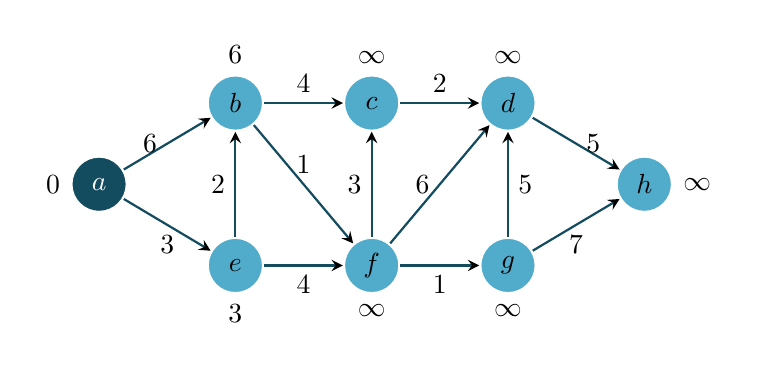
\begin{tikzpicture}[thick, main/.style = {draw=white, text=black, circle, fill=bluedot,rounded corners=0.5mm,minimum size=2em}, scale=0.2,
        selected/.style = {draw=white, text=white, circle, fill=darkblue,rounded corners=0.5mm,minimum size=2em}]
        \matrix [column sep=1cm, row sep=0.3cm]{
                           & \node[main,label=above:{$6$}] (2) {$b$}; & \node[main,label=above:{$\infty$}] (5) {$c$}; & \node[main,label=above:{$\infty$}] (8) {$d$};  &  \\
    \node[selected,label=left:{$0$}] (1) {$a$}; & & & & \node[main,label=right:{$\infty$}] (11) {$h$}; \\ 
     & \node[main,label=below:{$3$}] (3) {$e$}; & \node[main,label=below:{$\infty$}] (6) {$f$}; & \node[main,label=below:{$\infty$}] (9) {$g$}; \\ 
    };
    \draw[-stealth, draw=darkblue, thick] (1) edge node [left] {6} (2);
    \draw[-stealth, draw=darkblue, thick] (1) edge node [below] {3} (3);
    \draw[stealth-, draw=darkblue, thick] (2) edge node [left] {2} (3);
    \draw[-stealth, draw=darkblue, thick] (2) edge node [above] {4} (5);
    \draw[-stealth, draw=darkblue, thick] (3) edge node [below] {4} (6);
    \draw[stealth-, draw=darkblue, thick] (5) edge node [left] {3} (6);
    \draw[-stealth, draw=darkblue, thick] (5) edge node [above] {2} (8);
    \draw[-stealth, draw=darkblue, thick] (6) edge node [below] {1} (9);
    \draw[-stealth, draw=darkblue, thick] (2) edge node [above] {1} (6);
    \draw[-stealth, draw=darkblue, thick] (6) edge node [left] {6} (8);
    \draw[stealth-, draw=darkblue, thick] (8) edge node [right] {5} (9);
    \draw[-stealth, draw=darkblue, thick] (8) edge node [right] {5} (11);
    \draw[-stealth, draw=darkblue, thick] (9) edge node [below] {7} (11);
    \end{tikzpicture}
\end{center}
    
\end{document}